\chapter{Ferramenta desenvolvida}

Neste trabalho foi desenvolvido um protótipo cujo objetivo é auxiliar na interpretação de exames de tomografia computadorizada pulmonares. O protótipo, através do processamento de imagens digitais e de técnicas de recuperação de imagens baseada em conteúdo, é capaz de oferecer suporte ao médico na realização do diagnóstico do paciente.

Neste capítulo serão demonstrados aspectos da implementação e utilização do protótipo desenvolvido.

\section{Ambiente de desenvolvimento}

O desenvolvimento do trabalho foi realizado utilizando-se um notebook equipado com processador Intel\textregistered~Core\texttrademark~2~Duo T5450 (1.66GHz), 3GB de memória RAM DDR2 e placa de vídeo NVIDIA\textregistered~GeForce\texttrademark~8400M~GS com 256MB de memória dedicada.

O sistema operacional de desenvolvimento foi o GNU/Linux da distribuição Debian \textit{testing}, utilizando a IDE NetBeans 6.1 com o auxílio das ferramentas cmake, make e gcc. Todas as ferramentas utilizadas são multiplataforma.

\section{Imagens utilizadas}

Nos diversos experimentos executados durante o desenvolvimento da ferramenta, foram utilizadas imagens médicas de tomografia computadorizada pulmonar cedidas pelo Hospital das Clínicas da Faculdade de Medicina de Ribeirão Preto da Universidade de São Paulo (HCFMRP – USP).

% TODO: como foram obtidas, especificações da máquina

\section{Linguagens de programação}

Para o desenvolvimento da ferramenta foram utilizadas as linguagens de programação C++, PHP e javascript. O C++ é uma linguagem de alto nível de abstração, com sistema de tipos estático e que permite a programação em múltiplos paradigmas, incluindo programação procedural, genérica e orientada a objetos \cite{stroustrup2000}. Esta linguagem foi desenvolvida originalmente por Bjarne Stroustrup nos laboratórios Bell como uma melhoria para a linguagem de programação C. Dentre as capacidades do C++, destacam-se a possibilidade de fazer abstração de dados, a sobrecarga de operadores e métodos e tratamento de exceções.

Esta linguagem foi escolhida devido a seu desempenho, suporte a orientação a objetos e velocidade de desenvolvimento, além de ser a linguagem nativa da biblioteca mais utilizadas, a ITK.

Já as linguagens PHP e javascript foram escolhidas para a interface gráfica com o usuário (GUI), pois permitem que a ferramenta esteja disponível pela internet, tornam a centralização do banco de dados muito mais fácil, compartilhando o contínuo treinamento da ferramenta e não exigem que a máquina do usuário tenha grande poder de processamento.

\section{Bibliotecas}

Muitas das funções desempenhadas pela ferramenta desenvolvida incluem o processamento e visualização de imagens e gráficos, e ainda a construção, treinamento e utilização de uma rede neural. O desenvolvimento destas rotinas foi escrito com base em algumas bibliotecas que são referência na área por proverem grande quantidade de algoritmos já codificados, testados e prontos para o uso.

Todas as bibliotecas utilizadas no desenvolvimento da ferramenta são distribuídas livremente, com código-fonte aberto. Além disso todas as bibliotecas são multiplataforma.

\subsection{ITK}

Insight Segmentation and Registration ToolKit (ITK) é uma biblioteca proposta pela Biblioteca Nacional de Medicina dos Estados Unidos da América, voltada para segmentação e registro de imagens \cite{yoo}.

a biblioteca é composta por algoritmos e estruturas de representação de dados com duas finalidades principais: a identificação e classificação de elementos encontrados em uma imagem digital (segmentação) e a tarefa de alinhar imagens ou encontrar correspondências entre dados (registro).

No ITK há um foco em aplicações médicas, embora não haja restrições quanto ao processamento de outros tipos de dados. Essa biblioteca não dá enfoque à parte de visualização deixando a cargo de outras ferramentas que possam ser utilizadas conjuntamente, como o VTK.

O ITK é mantido, basicamente, por seis instituições: Kitware, GE Corporate R\&D, Insightful, University Chapel Hill, University of Utah e University of Pennsylvania, sendo as três primeiras comerciais e as demais são instituições acadêmicas. Outros membros do projeto são Harvard Brigham \& Women's Hospital, University of Pittsburgh e Columbia University \cite{itk-page}.

Quanto à linguagem, ITK também é escrito em C++, mas possui interface para utilização a partir de outras linguagens. É um conjunto de ferramentas que provê uma grande quantidade de algoritmos pré-codificados e testados para fazer registro e segmentação de imagens, bem como rotinas para leitura e decodificação de diversos padrões de arquivos.

O ITK é também distribuído livremente, com código-fonte aberto e uma licença bem semelhante à do VTK, impondo poucas restrições ao seu uso, modificação e distribuição.

\subsection{FANN}

Fast Artificial Neural Network (FANN) é uma biblioteca de RNAs open source. Ela é simples, bem documentada, versátil, fácil de usar e rápida. A FANN é implementada em C, mas possui versões para C++, Java, Perl, PHP, Python, Ruby, Delphi, Haskel, Mathematica, Matlab, Prolog, Octave, Smalltalk e .NET. Ela foi desenvolvida por Steffen Nissen do departamento de Ciência da Computação da Universidade de Copenhagen, que, logo depois, liberou o código sob a licença GPL.

A escolha dessa biblioteca teve como fator principal a possibilidade de se utilizar as linguages C++ e PHP. O que não foi encontrado em nenhuma outra biblioteca.

A biblioteca implementa uma RNA de múltiplas camadas totalmente ou esparsamente conectada. Com a FANN, a criação de uma RNA é feita em três níveis. O primeiro é a descrição da rede, o segundo é a criação das conexões da primeira camada, e depois as interconexões das demais camadas. Ela pode trabalhar tanto com números em ponto flutuante quanto números inteiros. Além disso, ela possui um framework para que seja fácil o treinamento a partir de conjuntos da dados.

Ela é flexível, quase todos os valores dos algoritmos de treinamento podem ser alterados, assim como os próprios algoritmos de treinamento.

\section{Algoritmos}

Grande parte da construção da ferramenta foi constituída pelo desenvolvimento de algoritmos que desempenham as funções propostas. A seguir são apresentados, de modo simplificado, cada um dos algoritmos.

\subsection{Segmentação de imagens de tomografia computadorizada dos pulmões}

O objetivo deste algoritmo é gerar a partir de uma fatia da imagem de tomografia computadorizada, duas imagens contendo cada uma apenas um dos pulmões com as partes que não pertencem a eles pretas.

São 5 as etapas desse algoritmo:
\begin{enumerate}
 \item Realizar um threshold adaptativo, como explicado na subseção \ref{subsec:threshold}.
 \item Subtrair a região que não pertence ao corpo do paciente.
 \item Eliminar pequenas regiões erroneamente marcadas como pulmão pelo threshold.
 \item Eliminar buracos dentro do pulmão e juntar pedaços que possam ter ficado separados.
 \item Identificar cada um dos pulmões e se necessário separa-los.
\end{enumerate}

Para subtrair a região que não pertence ao corpo do paciente, são removidos todos os pixels que estão conectados e possuem o mesmo nível de cinza dos pixels da borda da imagem. Como demonstrado na fig.~\ref{fig:remocao}.

\begin{figure}[ht]
 \begin{center}
  \subfigure[Antes da remoção.]{
\includegraphics[width=2.9in]{imagens/TCpulmaoTHRESHOLDED.png}}
  \subfigure[Depois da remoção.]{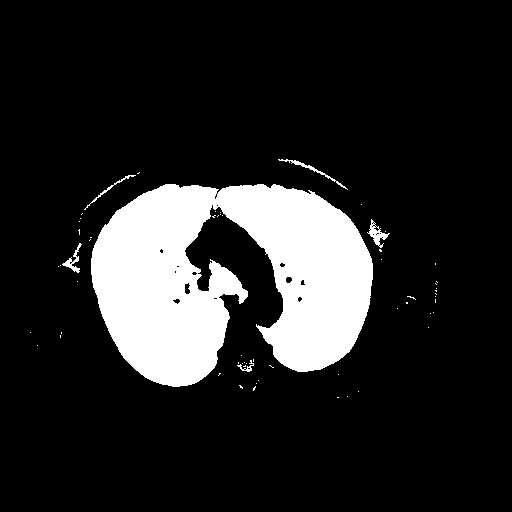
\includegraphics[width=2.9in]{imagens/TCpulmaoWOair.png}}
 \end{center}
 \caption{Imagem de TC antes e depois da remoção das partes que não pertencem ao corpo.}
 \label{fig:remocao}
\end{figure}

A eliminação das regiões que não fazem parte do pulmão é feita analisando-se todos os pixels que representam o pulmão (brancos) na imagem, de maneira que se a soma dos pixels vizinhos que representam o fundo (pretos) exceder em 2 ou mais a soma dos pixels vizinhos que representam o pulmão, então esse pixel se tornará parte do fundo. São considerados pixels vizinhos aqueles que se encontram no quadrado de 5x5 tendo como centro o pixel analisado.

Esse procedimento é realizado até 40 vezes, ou seja, ele será executado uma vez, se algum pixel for alterado, ele será executado novamente, até que nenhum pixel seja alterado ou que ele já tenha se repetido 40 vezes, podemos ver um exemplo na fig.~\ref{fig:clean}.

\begin{figure}[!ht]
 \begin{center}
  \subfigure[Antes da limpeza.]{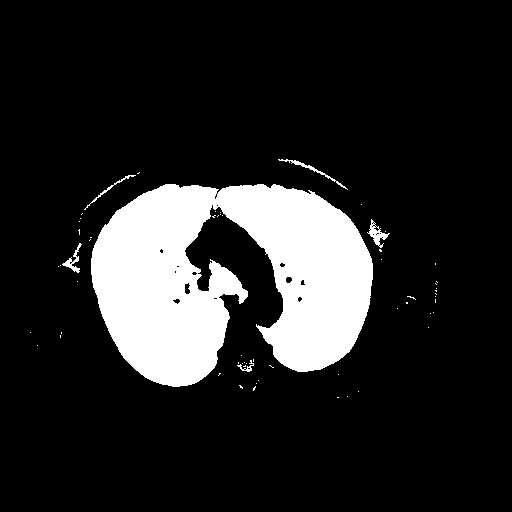
\includegraphics[width=2.9in]{imagens/TCpulmaoWOair.png}}
  \subfigure[Depois da limpeza.]{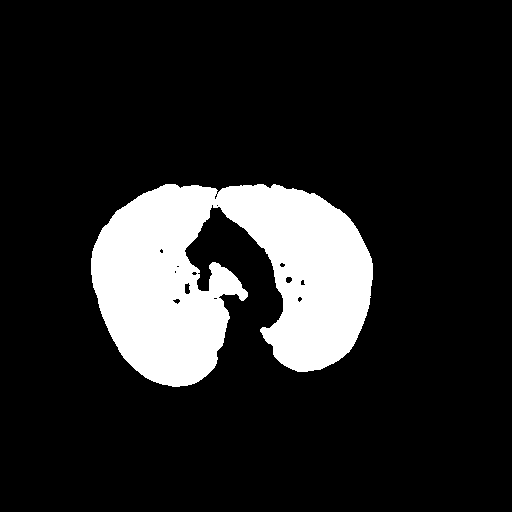
\includegraphics[width=2.9in]{imagens/TCpulmaoCleaning.png}}
 \end{center}
 \caption{Imagem de TC antes e depois da eliminação das regiões que não fazem parte do pulmão.}
 \label{fig:clean}
\end{figure}

Para remover os buracos dentro do pulmão e juntar pedaços separados de um mesmo pulmão, é realizado uma operação morfológica de fechamento utilizando como elemento estruturante um círculo de raio 6 pixels, como podemos ver na fig.~\ref{fig:fechamentoAplicado}. Essa operação pode causar com que pulmões muito próximos se juntem, tornando a próxima etapa ainda mais importante.

\begin{figure}[!ht]
 \begin{center}
  \subfigure[Antes do fechamento.]{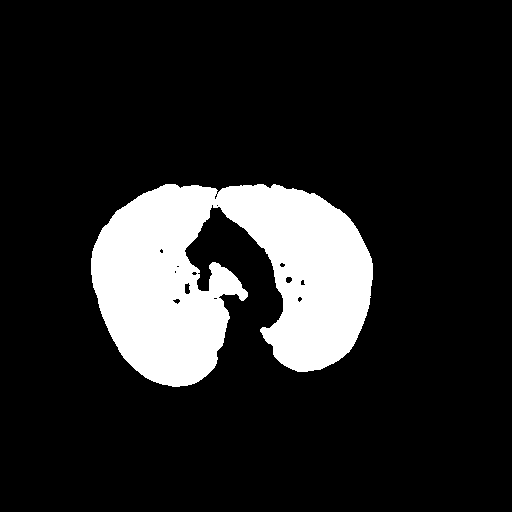
\includegraphics[width=2.9in]{imagens/TCpulmaoCleaning.png}}
  \subfigure[Depois do fechamento.]{
\includegraphics[width=2.9in]{imagens/TCpulmaoBinaryBall.png}}
 \end{center}
 \caption{Imagem de TC antes e depois da operação morfológica de fechamento utilizando um círculo de raio 6 pixels.}
 \label{fig:fechamentoAplicado}
\end{figure}

Para identificar os pulmões primeiro verifica-se quantas regiões conectadas existem, se existir apenas uma, realiza-se uma busca a partir do centro da imagem pela coluna que possuir menos pixels que representam o pulmão, sendo que a busca para quando a quantidade desses pixels começa a aumentar. Com essa estratégia paramos o algoritmo antes de encontrarmos estruturas pulmonares menores. Podemos ver um exemplo dessa etapa na fig.~\ref{fig:separacao}.

\begin{figure}[!ht]
 \begin{center}
  \subfigure[Pulmões juntos.]{
\includegraphics[width=1.9in]{imagens/TCpulmaoBinaryBall.png}\label{fig:separacao:a}}
  \subfigure[Pulmão esquerdo.]{
\includegraphics[width=1.9in]{imagens/TCpulmaoEsquerdo.png}\label{fig:separacao:b}}
  \subfigure[Pulmão direito.]{
\includegraphics[width=1.9in]{imagens/TCpulmaoDireito.png}\label{fig:separacao:c}}
 \end{center}
 \caption{Pulmões unidos em \ref{fig:separacao:a}, e depois devidamente separados e identificados em \ref{fig:separacao:b} e \ref{fig:separacao:c}.}
 \label{fig:separacao}
\end{figure}

\subsection{Recuperação de imagens baseada em conteúdo}

Primeiramente foi necessário escolher as características a serem utilizadas para o cálculo de similaridade, as quais foram energia, entropia, correlação, constraste e momento diferencial inverso.
% TODO: pq foram estas escolhidas?

Com isso é preciso que a RNA tenha 10 nodos de entrada, 5 para cada vetor de características. E como a saída da RNA é o valor de similaridade, ela possui apenas um nodo de saída. Para que tenhamos um valor entre 0 e 1 na saída, foi utilizada a seguinte função sigmóide:

\begin{equation}
	y = \frac{1}{1 + e^{-x}}
\end{equation}

A qual é derivada na equação~\ref{equa:sigmoide:derivada}, que tem custo computacional baixo, pois como utilizamos para aprendizado o algoritmo de retro-propagação, o valor de $y$ não precisa ser calculado novamente na atualização dos pesos.

\begin{equation}
	y \cdot (1 - y)
	\label{equa:sigmoide:derivada}
\end{equation}

A RNA foi dimensionada com 2 camadas intermediárias, sendo que na primeira camada temos 11 nodos e na segunda camada 13 nodos.

A taxa de aprendizado escolhida para o algoritmo de retro-propagação é 0,2. O valor de $o_j$, que é o valor de saída esperado, na equação~\ref{equa:back:output} é 1 se o usuário considerar as imagens comparadas similares, 0 se considerar diferentes e 0,5 se não for considerada igual nem diferente.

O treinamente é realizado com um conjunto de imagens de 20 pacientes. Que é repetido até 1000 vezes ou até que o erro médio do conjunto de imagens seja menor que 0,001. Alguns pares no conjunto de imagens de treinamento foram montados de modo a fazer com que a RNA seja associativa entre duas imagens, ou seja, se a similaridade de uma imagem $x$ com uma imagem $y$ for $z$, então a similaridade entre a imagem $y$ e a imagem $x$ também deve ser $z$. Também foram feitos pares no conjunto de imagens de treinamento com a mesma imagem, pois nesse caso o resultado deve ser, idealmente, 1.

\section{Interface Gráfica}

A ferramenta foi concebida para ser utilizada em dois modos, o modo normal e o modo de avaliação. No modo normal o usuário irá submeter uma imagem de TC pela página e escolher se quer ver as imagens mais similares ao pulmão esquerdo ou direito. Então ele poderá ver a segmentação feita nos dois pulmões da imagem enviada, e as 12 imagens mais similares ao pulmão escolhido (fig.~\ref{fig:lungRetriever}).

\begin{figure}[!htb]
 \begin{center}
  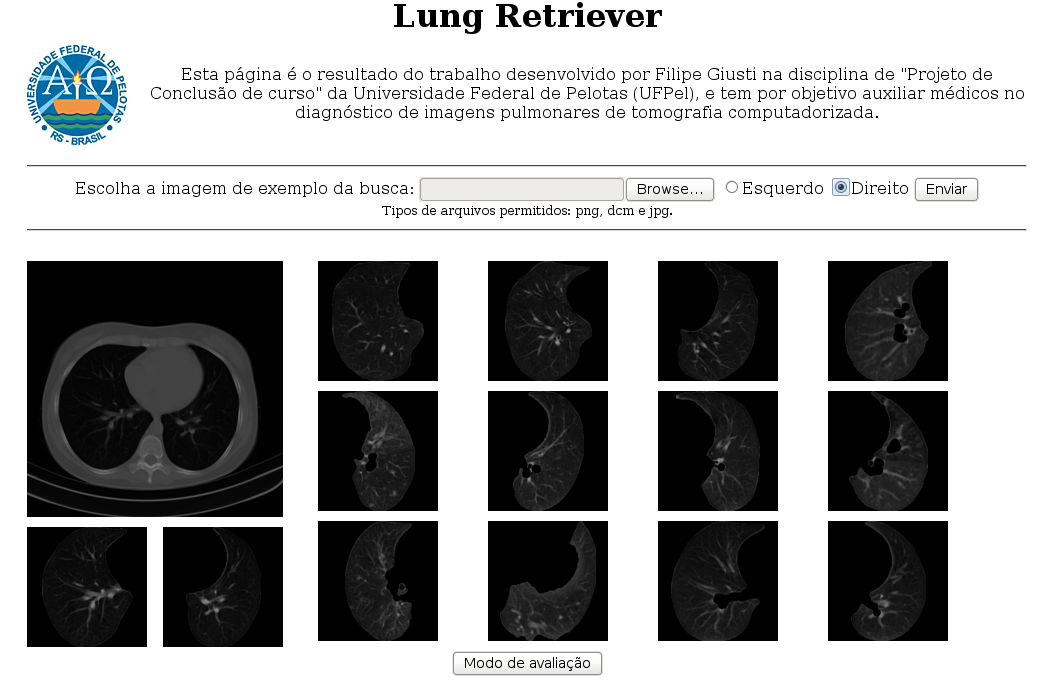
\includegraphics[width=5.8in]{imagens/LungRetriever.png}
 \end{center}
 \caption{GUI da ferramenta desenvolvida.}
 \label{fig:lungRetriever}
\end{figure}

Já no modo de avaliação o usuário irá ajudar a aperfeiçoar o sistema. Ele pode avaliar a relevância das imagens e submeter essa avaliação. Assim como também pode avaliar a segmentação feita na imagem enviada, mas que servirá apenas para ajudar a reavaliar o algoritmo de segmentação (fig.~\ref{fig:lungRetriever:aval}).

\begin{figure}[!htb]
 \begin{center}
  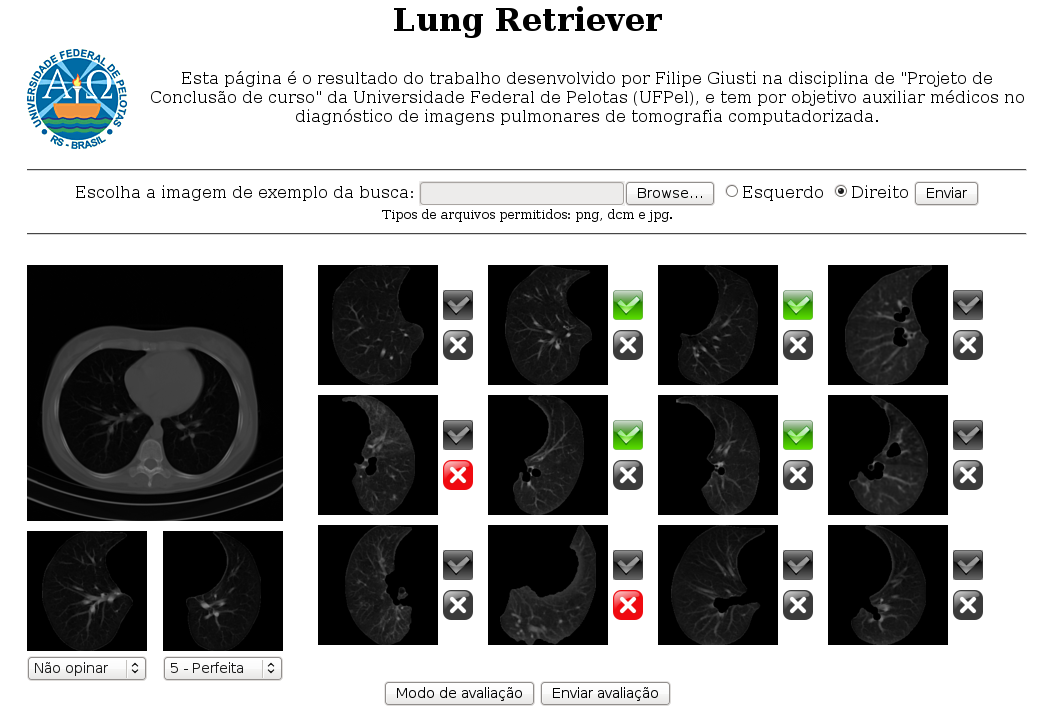
\includegraphics[width=5.8in]{imagens/LungRetrieverCOMaval.png}
 \end{center}
 \caption{GUI da ferramenta desenvolvida com o modo de avaliação ativado.}
 \label{fig:lungRetriever:aval}
\end{figure}